\documentclass[a4paper,12pt]{report}
\usepackage{titlesec}
\usepackage[T1]{fontenc}
\usepackage[utf8]{inputenc}
\usepackage[french]{babel}
\usepackage{enumitem}
\usepackage{pifont}
\usepackage{graphicx}
\usepackage{chngcntr} 
\usepackage{placeins}
\usepackage{float}
\usepackage{amssymb}
\usepackage{longtable}
\usepackage{array}
\usepackage{ragged2e}
\usepackage{booktabs}
\usepackage[table]{xcolor}
\usepackage[T1]{fontenc}
\usepackage[margin=1in]{geometry}

% Core packages
\usepackage{amsmath,amssymb}
\usepackage{tikz-cd}
\usetikzlibrary{calc}
\usepackage{tikzpagenodes}
\usepackage{eso-pic}
\usepackage{multicol}
\usepackage{array}
\usepackage{float}
\usepackage{tabularx}
\usepackage{ragged2e}

\newcolumntype{Y}{>{\RaggedRight\arraybackslash}X}
\newcolumntype{C}[1]{>{\centering\arraybackslash}p{#1}}


% Paragraphs
\setlength{\parindent}{0pt}
\setlength{\parskip}{1\baselineskip}
 % décale la numérotation des sections pour qu'elle ne dépende plus du chapitre
\definecolor{rowalt}{gray}{0.95}
\newcommand{\sone}{Sprint 1}
\newcommand{\stwo}{Sprint 2}
\newcommand{\sthree}{Sprint 3}
\newcommand{\phigh}{Haute}
\newcommand{\pmid}{Moyenne}
\newcommand{\plow}{Faible}
\renewcommand{\thesection}{\arabic{section}} % sections = 1,2,3...
\renewcommand{\thesubsection}{\thesection.\arabic{subsection}} 

% Page decoration: bandeau décoratif en haut de chaque page
\AddToShipoutPictureBG*{%
  \begin{tikzpicture}[remember picture, overlay]
    \fill[gray!10] ($(current page.north west)+(1cm,-0.8cm)$) rectangle ($(current page.north east)+(-1cm,-1.5cm)$);
    \draw[line width=0.5pt] ($(current page.north west)+(1cm,-0.8cm)$) rectangle ($(current page.north east)+(-1cm,-1.5cm)$);
  \end{tikzpicture}%
}

\begin{document}
\sloppy
\pagenumbering{gobble}

\tableofcontents
\newpage

\listoftables
\addcontentsline{toc}{chapter}{Liste des tableaux}
\newpage

\listoffigures
\addcontentsline{toc}{chapter}{Liste des figures}
\newpage

\pagenumbering{arabic}
\setcounter{page}{1}
\chapter*{Introduction générale}
\addcontentsline{toc}{chapter}{Introduction générale}

Aujourd'hui, l'obésité et les maladies liées à une mauvaise hygiène de vie constituent l'un des principaux défis de santé publique au niveau mondial. Devant la sédentarité croissante et les habitudes alimentaires déséquilibrées, de plus en plus de personnes cherchent des solutions efficaces pour reprendre le contrôle de leur santé, améliorer leur condition physique et adopter un mode de vie plus sain. C'est dans ce cadre que les plateformes numériques dédiées au fitness et à la nutrition se sont imposées comme des outils essentiels, permettant aux utilisateurs de bénéficier d'un accompagnement personnalisé et accessible pour suivre leurs activités physiques, gérer leur alimentation et atteindre leurs objectifs de bien-être.



Notre projet de fin d'études en vue de l'obtention du Diplôme de Mastère professionnel en Intelligence Artificielle et Internet des Objets, s'inscrit dans cette perspective. Notre objectif est de créer UFitPal, une plateforme intelligente de fitness et de nutrition. Ce projet vise à développer une application web permettant d'offrir un suivi personnalisé aux athlètes, de faciliter la collaboration avec des coachs sportifs et des nutritionnistes, et d'intégrer des modules d'intelligence artificielle pour optimiser les recommandations et
 modéliser les comportements des utilisateurs.

Ce rapport comprend les différentes étapes et tâches que nous avons accomplies lors de la réalisation de ce projet. Il comporte quatre chapitres :

\begin{itemize}[leftmargin=*, itemsep=4pt]
    \item Dans le premier chapitre, nous abordons le cadre général du projet en présentant l'organisme d'accueil, la description et les objectifs d'UFitPal, ainsi qu'une étude de l'existant et la méthodologie de travail adoptée.
    \item Le deuxième chapitre expose les acteurs du système, ainsi que les exigences fonctionnelles et non fonctionnelles de l'application, l'architecture technique retenue, le Product Backlog global et l'environnement de développement utilisé.
    \item Le troisième chapitre vise à présenter le Sprint 1, comprenant la conception et le développement des fonctionnalités d'authentification, de gestion des profils et de communication entre les différents acteurs de la plateforme.
    \item Le quatrième chapitre est consacré au Sprint 2, dédié au suivi sportif et nutritionnel de l'athlète, à la gestion des plans repas par le nutritionniste, ainsi qu'à l'intégration des modules d'intelligence artificielle, incluant les modèles prédictifs et le chatbot IA.
\end{itemize}

Enfin, une conclusion générale et perspectives résume le travail accompli et illustre les améliorations et extensions envisageables pour la plateforme UFitPal.

\newpage

\chapter*{Chapitre 1: Présentation du projet}  % Pas de numéro ajouté automatiquement
\addcontentsline{toc}{chapter}{Chapitre 1: Présentation du projet}  % Ajoute dans le sommaire

\section{Introduction du chapitre}
Dans ce chapitre, nous présentons le cadre général de notre stage au sein de HOLMENA Company for Digital Solutions. Nous introduisons l’entreprise d’accueil, ses domaines d’activité ainsi que les services qu’elle propose. Nous décrivons ensuite le projet réalisé et ses objectifs principaux. Enfin, l’étude de l’existant permet de cerner la problématique et de démontrer la valeur ajoutée de la solution développée.

\section{Présentation de l’organisme}

HOLMENA Company for Digital Solutions est une entreprise innovante fondée en 2024, spécialisée dans les solutions informatiques et numériques au sein de la région MENA.  
HOLMENA est une équipe jeune et pleine d'énergie réunie pour satisfaire les besoins de ses clients et les soutenir tout au long de leurs projets.
\begin{figure}[htbp]
    \centering
    
\includegraphics[width=0.5\textwidth]{images/image.jpeg}
    \caption{Logo de HOLMENA Company for Digital Solutions}
    \label{fig:holm}
\end{figure}

\FloatBarrier
\subsection{L’équipe de la société}

C’est une entreprise spécialisée dans les solutions digitales, le web et l’intelligence artificielle, dirigée par une équipe fondatrice dynamique et complémentaire :

\begin{itemize}
    \item Gérant (Fondateur \& Project Manager) : Mohamed Rashad Rouine
    \item Direction Générale
    \item Direction Technique
    \item Service Opérations Digitales (Co-Founder \& Digital Operations Specialist)
    \item Direction Stratégique (Co-Founder \& Chief Strategic Officer)
    \item Service Développement \& Croissance
    \item Service Design \& Communication (Chief Designer)
\end{itemize}

\subsection{Services}

\begin{itemize}
    \item Services digitaux et intégration de solutions numériques innovantes.
    \item Services de recherche et développement en technologies IT.
    \item Services de conception Web / mobile et développement d'applications performantes.
    \item Développement de solutions e-commerce sécurisées et évolutives.
    \item Services de création de contenu multimédia et gestion de présence digitale.
\end{itemize}

\section{Présentation du projet}

\subsection{Contexte du projet}
Dans le cadre de notre projet de fin d'études en vue de l'obtention du Diplôme de Mastère professionnel en intelligence artificielle \& internet des objets, j’ai effectué un stage à l’entreprise HOLMENA Company for Digital Solutions afin de concevoir et développer une plateforme innovante intitulée UFitPal : Assistance intelligente en fitness et nutrition.

\subsection{Description du projet}
Notre projet consiste à concevoir et développer une plateforme intelligente de fitness et de nutrition, capable d'offrir une expérience personnalisée et innovante aux utilisateurs grâce à l'intelligence artificielle. Elle propose des programmes d’entraînement et des plans nutritionnels personnalisés, qui s'adaptent aux besoins spécifiques de chaque utilisateur.

\subsection{Les objectifs}
Notre objectif est de créer une plateforme pour le fitness et la nutrition qui répondra aux besoins spécifiques du public MENA. En effet, l'application offre les services suivants :

\begin{itemize}[label=\ding{51}]
  \item Mettre en place des programmes d'entraînement complètement personnalisés en fonction du niveau physique, des objectifs et du rythme de vie de l'utilisateur.
   \item Proposer des recommandations alimentaires personnalisées qui respectent les besoins énergétiques, les objectifs de santé et le mode de vie de chaque utilisateur.
  \item Offrir des interfaces simples et intuitives pour les différents profils (athlète, coach, nutritionniste).
  \item Assurer l'intégrité, la sécurité et la cohérence des données à chaque mise à jour et insertion.
  \end{itemize}
\section{Étude de l’existant du projet}
L'analyse de l'existant se divise principalement en trois parties : la description de l'existant, la critique de l'existant et la solution suggérée.
\subsection{Description de l’existant du projet}
L'objectif de cette partie est d'examiner les solutions existantes dans le domaine 
des applications de fitness et nutrition afin de mieux cerner les besoins spécifiques du projet UFitPal, 
et de les intégrer de manière intelligente dans sa conception et son développement.

Nous avons donc examiné les applications les plus populaires disponibles à l'échelle mondiale et dans la région MENA.

Nous citons :

\begin{itemize}

\item \textbf{ArabFit} est une application mobile de fitness arabophone, disponible sur iOS et Android, 
destinée aux utilisateurs du Maghreb et de la région MENA. Elle est conçue pour aider les utilisateurs 
à développer leur musculature, perdre du poids et obtenir les meilleurs résultats grâce à des exercices 
physiques quotidiens.

\begin{figure}[H]
    \centering
    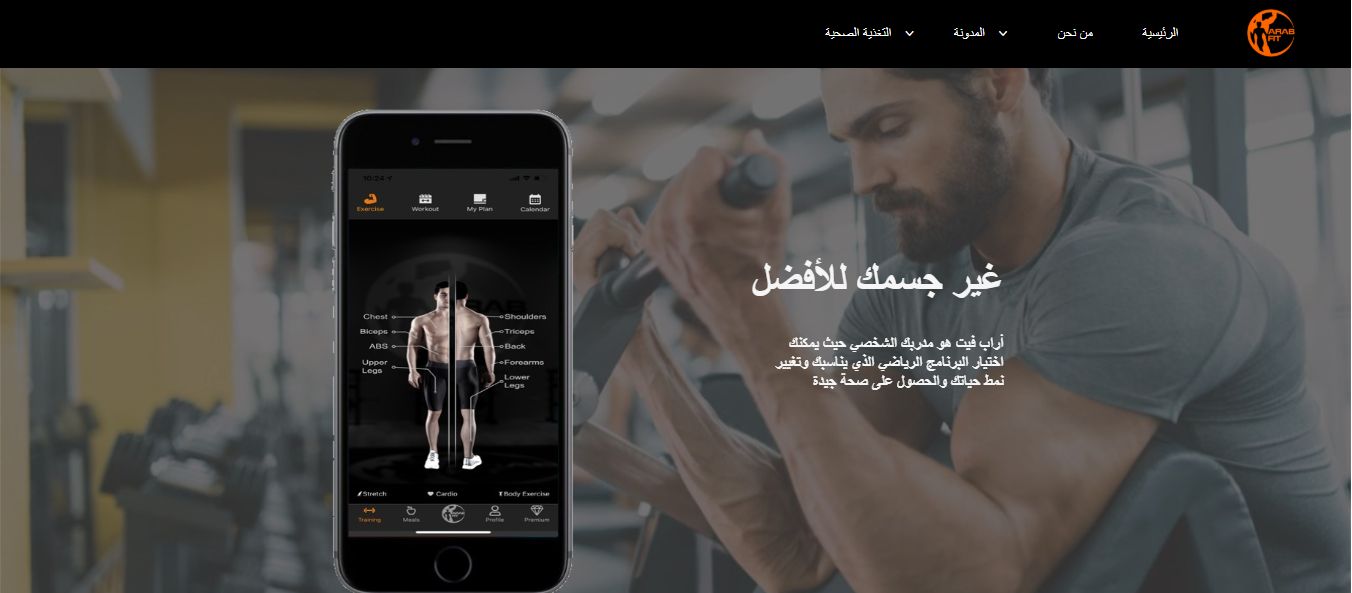
\includegraphics[width=1\textwidth]{images/arbfit.png}
    \caption{Interface de l'application ArabFit}
    \label{fig:arbfit}
    
\end{figure}

\FloatBarrier


\item \textbf{MyFitnessPal} est une application américaine de suivi nutritionnel et sportif, 
lancée en 2005 et rachetée par Under Armour en 2015. 

\begin{figure}[H]
    \centering
    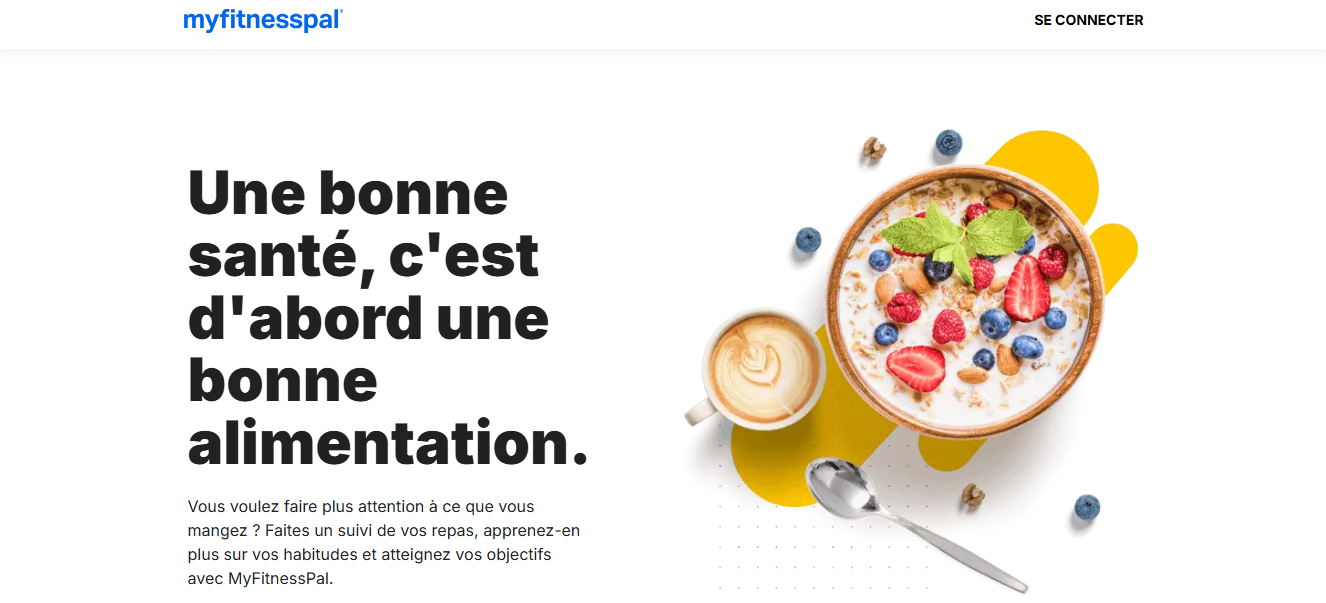
\includegraphics[width=1\textwidth]{images/myfitt.png}
    \caption{Interface de l'application MyFitnessPal}
    \label{fig:myfitnesspal}
    
\end{figure}
\vspace{-1cm} 
\FloatBarrier

\end{itemize}

\subsection{Problématique}
Comment concevoir et implémenter une plateforme numérique de santé préventive et intelligente qui unifie l'accompagnement humain (coachs et nutritionnistes), 
l'analyse métabolique et l'intelligence artificielle prédictive, afin d'offrir des recommandations ultra-personnalisées, de détecter de manière proactive les stagnations
 physiques et de maximiser l'adhésion à long terme des utilisateurs ? 

 
  
 
\subsection{Critique de l'existant}

L'objectif de cette étape est d'identifier les principales anomalies observées, 
pour analyser les causes profondes et trouver des solutions adaptées.
Dans notre étude, nous avons observé les éléments suivants :

\begin{itemize}[label=$\star$]
 \item  Personnalisation limitée, reposant sur des paramètres statiques (âge, poids, objectif calorique),
 sans moteur d'IA adaptatif capable d'évoluer en fonction des progrès de l'utilisateur.
 \item Aucun suivi nutritionnel n'est autorisé, sauf dans le cas d'une journalisation descriptive, 
 sans analyse intelligente ni recommandations personnalisées.
 \item Aucune dimension de relation professionnelle n'est intégrée : pas d'espace dédié à la relation athlète-coach ou athlète-nutritionniste, 
 ni de messagerie structurée, ni de module de planification de rendez-vous.
 \item Ces solutions ne contiennent aucune fonctionnalité d'intelligence artificielle avancée, telle que la prédiction d'évolution,
 la détection de plateau sportif ou un assistant de conseils personnalisés.
 \item Le suivi corporel est partiel, centré principalement sur le poids et les calories, sans intégration des métriques
 anthropométriques ni outils de visualisation de la progression.
 \end{itemize}
  


\subsection{Les solutions proposées}
Face aux défis identifiés dans l'étude de la situation existante,
 notamment la fragmentation des données et le manque d'adaptation aux spécificités de la région MENA,
  nous proposons une solution innovante baptisée UFitPal:

\begin{itemize}[label=$\star$]
\item  Mise en place de programmes sportifs et nutritionnels personnalisés en fonction du profil utilisateur (âge, objectifs, contraintes), 
grâce à un système d'intelligence artificielle adaptatif.

\item  Un espace professionnel dédié permettant au coach et au nutritionniste d'envoyer des invitations, de gérer leurs athlètes, 
de rédiger des notes de suivi, de créer des plans repas personnalisés et de planifier des rendez-vous .
\item Évaluation prédictive des performances grâce à des modèles de machine learning : score de risque d'abandon, prédiction d'évolution du poids, 
probabilité d'atteinte de l'objectif fitness et détection automatique des plateaux sportifs.
\item Un assistant chatbot IA disponible pour l'athlète afin d'obtenir des conseils personnalisés sur la nutrition et l'entraînement.
 \item Une interface ergonomique, intuitive et multilingue qui regroupe toutes les données pour éviter la dispersion et encourager l'adhésion à long terme.
\end{itemize}

\section{Méthodologie de travail}

\subsection{Choix d'une approche agile}
Pour le développement de l'application UFitPal, nous avons adopté une méthodologie agile afin de
 répondre aux exigences évolutives d'un projet numérique innovant. Les approches agiles, contrairement 
 aux approches traditionnelles en cascade, favorisent des cycles de développement courts et itératifs 
 qui permettent une adaptation rapide aux retours des utilisateurs et aux contraintes techniques rencontrées tout au long du projet.

\subsection{Méthodologie adoptée : Scrum}
Parmi les cadres agiles disponibles, nous avons choisi Scrum pour sa structure bien définie et sa capacité à organiser efficacement le travail en équipe.
 Dans le cadre du projet UFitPal, cette méthodologie nous a permis de livrer des incréments fonctionnels à chaque sprint,
  tout en conservant une vision globale du produit final.

\subsubsection{Organisation de l'équipe}
L'équipe projet a été structurée selon les rôles Scrum suivants :
\begin{itemize}
    \item \textbf{Product Owner} : chargé de recueillir les besoins des utilisateurs cibles 
    (sportifs, coachs) et de prioriser les fonctionnalités du backlog en fonction de leur 
    valeur métier.
    \item \textbf{Scrum Master} : responsable du respect du cadre Scrum, de la levée des 
    obstacles et de la fluidité des cérémonies.
    \item \textbf{Équipe de développement} : constituée de développeurs front-end et back-end, 
    d'un designer UI/UX et d'un spécialiste en intelligence artificielle, assurant la 
    réalisation technique des fonctionnalités définies.
\end{itemize}

\subsubsection{Artefacts utilisés}
Les artefacts Scrum suivants ont structuré notre gestion du projet :
\begin{itemize}
    \item \textbf{Product Backlog} : liste vivante et priorisée de l'ensemble des 
    fonctionnalités d'UFitPal, alimentée en continu par les retours utilisateurs et les 
    évolutions des besoins.
    \item \textbf{Sprint Backlog} : sous-ensemble du Product Backlog sélectionné à chaque 
    début de sprint, découpé en tâches assignées aux membres de l'équipe.
    \item \textbf{Incrément} : version fonctionnelle et testable de l'application livrée 
    à l'issue de chaque sprint, enrichissant progressivement les fonctionnalités de la 
    plateforme.
\end{itemize}

\subsubsection{Cérémonies pratiquées}
Afin d'assurer un suivi régulier et une communication efficace au sein de l'équipe, nous 
avons mis en place les cérémonies Scrum suivantes :
\begin{itemize}
    \item \textbf{Sprint Planning} : tenue en début de chaque sprint pour définir les 
    objectifs à atteindre et répartir les tâches entre les membres de l'équipe.
    \item \textbf{Daily Scrum} : point quotidien de quinze minutes permettant à chaque 
    membre de partager son avancement, ses blocages et ses objectifs du jour.
    \item \textbf{Sprint Review} : présentation de l'incrément réalisé aux parties 
    prenantes afin de valider les fonctionnalités développées et d'ajuster les priorités.
    \item \textbf{Sprint Retrospective} : réunion d'équipe visant à analyser le déroulement 
    du sprint écoulé, à capitaliser sur les bonnes pratiques et à corriger les 
    dysfonctionnements identifiés.
\end{itemize}

\subsection{Organisation en sprints}
Le projet UFitPal a été découpé en sprints d'une durée de deux semaines chacun. Cette 
cadence nous a permis de maintenir un rythme de livraison régulier tout en intégrant 
progressivement les fonctionnalités clés de l'application, depuis la gestion des profils 
utilisateurs jusqu'à l'intégration du module d'intelligence artificielle. Le détail des 
sprints réalisés et de leurs livrables est présenté dans la section suivante.


\section{Conclusion }
Ce chapitre a présenté une perspective globale de la société d'accueil, analysé des applications 
existantes aux fonctionnalités similaires à celles que nous voulons développer, et exposé la 
méthodologie de travail adoptée.Dans le prochain chapitre, nous procédons à la 
spécification des besoins fonctionnels et non-fonctionnels, à la définition de l'architecture 
technique de l'application, ainsi qu'à la présentation du Product Backlog global et de 
l'environnement de travail retenu.

\chapter*{Chapitre 2 : Réalisation de l'Application}
\addcontentsline{toc}{chapter}{Chapitre 2 : Réalisation de l'Application}

\setcounter{section}{0}
\section{Introduction du chapitre}
Ce chapitre traite de la spécification des besoins du projet UFitPal, une étape cruciale pour s'assurer 
que les objectifs de la plateforme correspondent aux attentes des utilisateurs.
 Il comporte l'analyse des besoins fonctionnels et non fonctionnels, le diagramme global des cas d'utilisation, 
 l'architecture de l'application, le Product Backlog général et l'environnement de travail adopté. 
 Ces différents éléments constituent une vision claire et structurée du projet, 
 et offrent donc une base solide pour sa conception, son développement et son évolution future.
 \section{ Analyse des besoins}


\end{document}